% Created 2019-12-07 Sat 01:19
% Intended LaTeX compiler: pdflatex
\documentclass[a4paper, 11pt]{extarticle}
             \usepackage[utf8]{inputenc}
\usepackage[left=2cm, right=2cm, bottom=2.5cm, top=2.5cm]{geometry}
% Paquetes de matemáticas
\usepackage{amsmath, amsfonts, amssymb, commath}
\usepackage{tikz}
\newcommand{\tikzcircle}[2][red,fill=red]{\tikz[baseline=-0.5ex]\draw[#1,radius=#2] (0,0) circle ;}%
% Ajustes de idioma, gráficos, etc
\usepackage{adjustbox}
\usepackage{float}
\usepackage{hyperref}
\usepackage{graphicx}
\usepackage{gensymb}
\usepackage[spanish, english]{babel}
\usepackage{tikz}
\usepackage{multicol}
\usepackage{listings}
\usepackage{enumitem}
\setlist{nolistsep}
\usepackage{booktabs}
\usepackage{xcolor}
\usepackage{wrapfig}
%Fuentes.
% Alegreya tiene este toque antiguo con serifa, y la tipografía de las ecuaciones es también interesante.
% Gillius no tiene serifa, y también es equilibrada.
\usepackage[T1]{fontenc}
%\usepackage[default]{gillius}
\usepackage{newpxtext, newpxmath}
% Paquete para añadir Creative Commons al final del documento
\usepackage[
type={CC},
modifier={by-nc-nd},
version={3.0},
]{doclicense}
% Propiedades de párrafo
\setlength{\parindent}{0em}
\setlength{\parskip}{1.1em}
\renewcommand{\baselinestretch}{1.05}
\setlength\itemsep{0em}
% Definición de comandos. Muchos de ellos han surgido para Geometría, aunque se
% irá actualizando la lista. POSIBLEMENTE LO INTRODUZCA COMO COMANDOS DE ORG
\newcommand{\m}{\text{medio}}
\newcommand{\iso}{\text{Isom}}
% Para incluir mathcal en las ecuaciones. El /mathcal para Alegreya es el viejo
% y floritural estilo que odio.
\usepackage{calrsfs}
\DeclareMathAlphabet{\pazocal}{OMS}{zplm}{m}{n}
% Definición de colores agradables a la vista
\definecolor{azul}{HTML}{107896}
\definecolor{naranja}{HTML}{C2571A}
\definecolor{rojo}{HTML}{9A2617}
\definecolor{amarillo}{HTML}{BCA136}
\definecolor{verde}{HTML}{829356}
\definecolor{gris}{HTML}{909090}
\definecolor{rosa}{HTML}{F9A7B0}
\definecolor{amarillochillon}{HTML}{FBB117}
% Definición de comandos para teoremas, etc. El comando también incluye
% como argumento un texto, del estilo Teorema 3.5
\newcommand{\axioma}[1]{\textcolor{naranja}{\textbf{Axioma #1}}}
\newcommand{\tma}[1]{\textcolor{rojo}{\textbf{Teorema #1}}}
\newcommand{\propo}[1]{\textcolor{rojo}{\textbf{Proposición #1}}}
\newcommand{\defi}[1]{\textcolor{azul}{\textbf{Definición #1}}}
\newcommand{\obs}[1]{\textcolor{verde}{\textbf{Observación #1}}}
\newcommand{\ejem}[1]{\textcolor{verde}{\textbf{Ejemplo #1}}}
\newcommand{\ej}[1]{\textcolor{amarillo}{\textbf{Ejercicio #1}}}
\newcommand{\lema}[1]{\textcolor{rosa}{\textbf{Lema #1}}}
\newcommand{\cor}[1]{\textcolor{rosa}{\textbf{Corolario #1}}}
% La demostración es igual pero va con una letra más pequeña y en gris.
\newcommand{\dem}[1]{\textcolor{gris}{\small{Demostración. #1}}}
% Esto pone un triangulito de peligro para cuando algo es importante.
\newcommand{\importante}{\tikzcircle[amarillo, fill=amarillo]{4pt}\,}
% Para usar columnas emplea este trozo de código
% \begin{multicols*}{2}
% [\section{Axiomas para la geometría euclidiana plana}]
% 	\axioma{P1} Si tenemos el conjunto $\P$, denominado \textbf{plano}, y la aplicación $d:\P \times \P \rightarrow \R$ llamada \textbf{distancia}, entonces$(\P, d)$ es un espacio métrico.

\defi{2.2} Una \textbf{recta} $r \subset \P$ satisface
\begin{itemizex}
	\item $r$ contiene al menos dos puntos.
	\item Para toda terna de puntos $A, B, C$, están alineados si están en $r$.
\end{itemizex}

\axioma{P2} $\P$ contiene al menos tres puntos no alineados; y por dos puntos distintos, $A$ y $B$ de $\P$ pasa una recta, $r_{AB}$.

\defi{2.6} / \tma{2.7} Dos rectas se cortan si sólo tienen un punto en común, y si no tienen ningún punto en común, entonces se denominan \textbf{paralelas}, y se denota por $a \parallel b$. Dos rectas, o se cortan o son paralelas.

\importante\axioma{P3} Para toda recta $r \subset \P$ existe una biyección $\gamma: r \rightarrow \R$ tal que $|\gamma(X) - \gamma(Y)| = |x - y| = d(X, Y) \;\; \forall \;\; X,Y \in r$ 

\obs{2.8} Si $A, B \in r$ son distintos, entonces existe un punto $M\in r: d(A,M) = d(M,B)$ que denotamos por $\m[A,B]$ y se llama \textbf{punto medio}. Asimismo sólo existe un punto $B \in r$ tal que $B = \m[A, M]$.

\obs{2.9} Si $r$ es una recta y $P \in r$, entonces $r$ se puede dividir en dos \textbf{semirrectas}, que son los conjuntos $\{X \in r \; | \; \gamma(X) > \gamma(P)\}$ y $\{X \in r \; | \; \gamma(X) < \gamma(P)\}$.

\axioma{P4} Para toda recta $r \subset \P$ hay dos subconjuntos $H^1$ y $H^2$, denominados \textbf{semiplanos} de $r$, que verifican:
\begin{itemizex}
	\item $H^1 \cup H^2 = \P-r$
	\item Si $X,Y \in H^i$ entonces $[X,Y] \subset H^i$
	\item Si $X \in H^1$ y $Y \in H^2$ entonces $[X,Y] \cap r \neq \emptyset$.
\end{itemizex}

\defi{2.15} Sean $P, Q, R$ no alineados, entonces el triángulo $\triangle\{P,Q,R\}$, o $\triangle PQR$ está formado por los segmentos $[P,Q]$, $[Q,R]$, $[P,R]$, llamados lados, y los vértices $P,Q, R$.

\tma{2.16 [Axioma de Pasch]a} Dado un triángulo $\triangle PQR$ y una recta $r$; si $r$ corta a $[P,Q]$, entonces o corta a $[P,R]$ o a $[Q, R]$.

\defi{2.17 = 1.5} Una \textbf{isometría} en $\P$ es una biyección $g: \P \rightarrow \P$ que cumple que $d(g(X), g(Y)) = d(X,Y) \;\;\forall\;\; X,Y \in \P$.

\tma{2.18} Si $A,B \in \P$ y $g \in \iso(\P)$ entonces $g([A,B]) = [g(A), g(B)]$ y $g(r_{AB}) = r_{g(A)g(B)}$ 

\axioma{P5} Si $A_1, A_2 \in \P$ y $B_1, B_2 \in \P$ son dos pares de puntos que cumplen $d(A_1,A_2) = d(B_1,B_2)$ entonces existe $g \in \iso(\P)$ tal que $g(A_i) = B_i$. Se dice que esos pares de puntos son \textbf{congruentes}.

\axioma{P6} Para toda recta $r$ existe una isometría $\sigma$ llamada \textbf{reflexión} tal que  
\begin{itemizex}
	\item $\sigma(X) = X\iff X \in r$
	\item $\sigma \circ \sigma = \text{Id}$
\end{itemizex}


\defi{2.23} / \tma{2.25} / \cor{2.30} Una recta $l$ es \textbf{ortogonal} a $r$ si para todo $S \in l$ y para todo par de puntos $A, B$ que cumple que $M = \m[A,B]$, de modo que $l \cap r = M$, entonces se da que $d(A,S) = d(S,B)$. Se denota $l \perp_M r$. En estas condiciones, $l = \{X \in \P \; | \; d(S,A) = d(S,B)\}$, se denomina \textbf{mediatriz} de $[A,B]$. 

\begin{figure}[H]
	\centering
	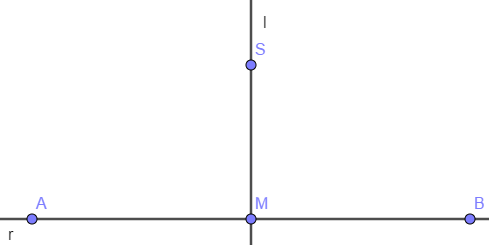
\includegraphics[width=7cm]{figuras/2-23.png}
	\vspace{-1em}
\end{figure}

\lema{2.21} Si $\sigma_r$ entonces, para todo $X$, $\m[X, \sigma_r(X)] \in r$.

\obs{2.24} Si $l \perp r$ y $g \in \iso(\P)$ entonces $g(l) \perp g(r)$.

\importante\tma{2.26} Si $l, r \subset \P$ cortan en $M$ y $\sigma_l, \sigma_r$ son dos reflexiones de $l$ y $r$, entonces se cumple que $l \perp_M r \iff r \perp_M l \iff \sigma_r(l) = l \iff \sigma_l(r) = r$.

\importante\tma{2.27 / 2.29} Para toda recta $r$ y todo punto $S \in \P - r$, existe una recta $l$ ortogonal a $r$, que pasa por $S$. Si $r$ es una recta, y $M \in r$, entonces existe $l$ tal que $l \perp_M r$.

\axioma{P7} Para toda recta $r$ y todo punto $P$ existe sólo una recta \textbf{paralela} a $r$ que pase por $P$.

\tma{2.31 / 2.33} Si $a \perp l$ y $b \perp l$ entonces $a \parallel b$. Sean $a \parallel b$. Entonces, para todo $A \in a$, la única recta $l \perp_A a$ también es ortogonal a $b$.

\tma{2.32} Las rectas parallelas forman una relación de equivalencia.
\begin{itemizex}
	\item Reflexividad: $a\parallel a$
	\item Simetría: $a \parallel b \rightarrow b \parallel a$
	\item Transitividad  $a \parallel b $ y  $b \parallel c \rightarrow a \parallel c$
\end{itemizex}

\ej{2.6} Sean $A,B \in r$, $A \neq B$. Para todo $t$, existe un único $P_t\in r$ que cumple $d(P_t,A) = \abs{t}$ y $d(P_t, B) = \abs{t-d(A,B)}$. En definitiva, la posición de $P_t$ está sólamente determinada por las distancias $d(A, P_t)$ y $d(P_t, B)$.
	 
	 
	 
	 
	 
	 
	 \end{multicols*}\pagebreak
% multicols* obliga a terminar una columna antes de empezar la siguiente.
\DeclareMathAlphabet{\pazocal}{OMS}{zplm}{m}{n}
\let\mathcal\pazocal
\usepackage{fancyhdr}
\pagestyle{fancy}
\lhead{Alex Martínez Ascensión}
\chead{}
\rhead{\today}
\date{}
\title{\Huge\vspace{-1em}Topología}
\hypersetup{
 pdfauthor={},
 pdftitle={\Huge\vspace{-1em}Topología},
 pdfkeywords={},
 pdfsubject={},
 pdfcreator={Emacs 26.2 (Org mode 9.2.5)}, 
 pdflang={English}}
\begin{document}

\maketitle
\vspace{-8em}

\section{Espacios topológicos}
\label{sec:org1412390}
Se dice que \(p\) es el límite de una sucesión de reales \(a_1, \cdots, a_n\) cuando, para todo abierto \(p - \epsilon, p + \epsilon\), existe un \(m\)
tal que para todo \(n \ge m\) se cumple que \(a_n \in (p- \epsilon, p +
\epsilon)\). 

Esta noción de intervalo se unifica en el concepto \textbf{bola}, y se define la familia
de intervalos de un punto \(p\), \(B(p)\). Sea \(X\) no vacío, para cada
\(p \in X\) existe una familia \(B(p)\). Se dice que \(B(p)\) es una \textbf{base
de entornos abiertos} de \(p\) si todas las familias \(B(p)\) verifican:
\begin{itemize}
\item B1: si \(U \subset B(p)\), entonces \(p \in U\).
\item B2: si \(U \in B(p)\) y \(V \in B(p)\), existe \(W \in B(p)\) tal que \(W \subset U \cap V\).
\item B3: si \(U \in B(p)\), para todo \(q \in U\) existe \(V \in B(q)\) tal
que \(V \subset U\).
\end{itemize}

Esta generalización de conjuntos \((p - \epsilon, p+\epsilon\) nos simplifica
y permite expandir la definición de topología, independientemente de una métrica
o distancia.

Se llama un \textbf{espacio métrico} \((X,d)\) a un conjunto \(X\) con una distancia
\(d\) definida en él. En un espacio métrico se llama \textbf{bola abierta} de centro
\(p\) y radio \(r\) al conjunto \(E(p,r) = \{ t \in X \;|\; d(p,t) < r \}\).
Las familias \(B(p)\) de todas las bolas con radios reales cumplen los puntos
B1, B2 y B3, por lo que constituyen base de entornos abiertos en \((X,d)\).

Si \(X\) es un conjunto en el que se ha definido un sistema de bases de
entornos abiertos \(B(p)\), un subconjunto \(A \subset X\) es un \textbf{conjunto abierto} cuando es \(\emptyset\) o cuando para cada \(t \in A\) existe un subconjunto \(U \in B(t)\) tal que \(U \subset A\).

En \(\mathbb{R}\) la topología usual (\(T_u\)) viene dada por \(B(p) =
(p - \epsilon, p + \epsilon)\). En esta topología, \((\mathbb{R}, T_u)\),
cada intervalo abierto \((a,b)\) viene dado como \(B(t), t = \frac{a+b}{2}\). El intervalo \([a,b)\) no es abierto, pues para \(a\) no existe ningún
conjunto \(U \in B(a)\) tal que \(U \subset [a,b)\).

Dos sistemas de bases de entornos abiertos, \(B(p), B'(p)\) son \textbf{equivalentes}
cuando determinan la misma topología \(T\) en \(X\); es decir, que para cada
\(U \in B(p)\) existe un \(U' \in B'(p)\) tal que \(U \subset U'\) y que para cada \(V' \in B'(p)\) exista un \(V \in B(p)\) tal que \(V'
\subset V\).

\subsection{Propiedades de una topología}
\label{sec:orgb7d0d4e}
Sea un conjunto \(X\). La topología \(T\) determinada en \(X\) cumple:
\begin{itemize}
\item P1: \(\emptyset \in T\) y \(X \in T\).
\item P2: Dada una familia de abiertos \(U_\lambda, \lambda \in L\) de \(T\), la
unión de los elementos, \(\bigcup_{\lambda} U_\lambda\) es un elemento de \(T\).
\item P3: Dada una familia \textbf{finita} \(U_i, i=1, \cdots, n\) de elementos de \(T\), la
intersección de los elementos, \(\bigcap_{i=1}^{n}U_i\) es un elemento de \(T\).
\end{itemize}

Un \textbf{espacio topológico} \((X, T)\) es un conjunto no vacío con una topología
definida en él. Una familia de subconjuntos de \(X\), \(H(p)\) para cada \(p \in X\) [SEAN DISCRETOS O CONTINUOS], si
cumple P1, P2, P3 entonces, las familias \(H\) forman una topología \(T\) en
\(X\). Si para esa topología existe una métrica \(d\), entonces decimos que
es una \textbf{topología metrizable}.

Si \(T, T'\) son dos topologías de \(X\), y \(T \subset T'\), entonces se dice que \(T\) es menos \textbf{fina} que \(T'\). La topología más
fina de todas es la \textbf{topología trivial}, dada por \(\{ \emptyset, X \}\), y la
menos fina, o \textbf{discreta}, está dada por \(\mathcal{P}(X)\), es decir, el
conjunto partición de \(X\). 

En \((X, T)\) se llama \textbf{conjunto cerrado} a un conjunto \(M \subset X\) tal que \(X-M\) es 
abierto. Una familia de conjuntos cerrados es \((X,T)\) verifica:
\begin{itemize}
\item C1: \(\emptyset \in T\) y \(X \in T\) son cerrados.
\item C2: Dada una familia \textbf{finita} de cerrados \(M_\lambda, \lambda \in L\) de \(T\), la
unión de los elementos, \(\bigcup_{\lambda} M_\lambda\) es un cerrado.
\item C3: Dada una familia \(M_\lambda, \lambda \in L\) de elementos de \(T\), la
intersección de los elementos, \(\bigcap_{L}U_\lambda\) es un elemento de \(T\).
\end{itemize}

Si \((X,T)\) es un estacio topológico y \(M \subset X\), la topología \(T_M = \{ M \cap U \}\) de las intersecciones de \(M\) con
abiertos \(U\) de \((X,T)\) se llama \textbf{topología inducida o subordinada} de \(T\). Así, el espacio \(M, T_M\) es un subespacio de \((X,T)\).

\section{Base de una topología}
\label{sec:org64c35c0}
Dada una topología \(T\) en \(X\), la \textbf{base de la topología}, \(B\), es una
familia de conjuntos tal que cualquier abierto no vacío \(U \subset T\) es una unión
 de elementos de \(B\). \(\forall U \subset
T\;,\; U = \cup_{i} B_i\)

Sea \(X\) un conjunto y \(F = \{ A_\lambda \}_{\lambda \in L}\) una familia
de subconjuntos de \(X\). Una condución necesaria y suficiente para que \(F\) sea 
base de \(X\) es:
\begin{itemize}
\item I: \(\bigcup_{\lambda}^{}\{ A_\lambda \} = X\)
\item II: Si \(A_\lambda, A_\mu\) son dos elementos de \(F\), y \(A_\lambda
  \cap A_\mu \neq \emptyset\), para cualquier
punto \(t \in  A_\lambda
  \cap A_\mu\) existe \(A_\nu \in F\) tal que \(t \in A_\nu\)
\end{itemize}


\subsection{1er y 2º axioma de numerabilidad}
\label{sec:orgdf32e2c}
Un espacio \((X,T)\) verifica el 1er axioma de numerabilidad si para todo \(x
\in X\) 
existe una base de entornos de \(x\) que sea numerable. Un espacio 
\((X,T)\) verifica el 2º axioma de numerabilidad cuando su topología
tiene una base numerable.

\subsection{Topología engendrada for una familia de subconjuntos}
\label{sec:org8acde8c}

Cualquier familia \(\{ A_\lambda \}\) de \(X\) que cumpla I es una subase de
una topología de \(X\). Si \(H = \{ A_\lambda \}\) cumple I y II, la familia \(B\) formada por las
 intersecciones (y uniones) finitas de \(H\) es base para alguna
topología de \(X\) y se llama \textbf{topología engendrada}. 


\section{Entornos en un espacio topológico}
\label{sec:orge4ce068}
Sea \((X,T)\) un espacio topológico, y \(p \in X\). \(A \subset X\) es entorno de \(p\) si existe un abierto \(U\) de la topología \(T\) tal que \(p \in U \subset A\). No todo entorno ha de ser abierto. Por ejemplo, \([0, 1)\) es entorno de
\(1/2\) (existe \(U = (1/2-1/4, 1/2+1/4) \subset [0, 1)\), pero no de \(0\) (ningún abierto en \(T\) cumple \(U \subset [0,1)\).

Los sistemas de entornos \(E(p)\) para \(X\) cumplen:
\begin{itemize}
\item E1: Si \(A \in E(p)\), entonces \(p \in A\).
\item E2: Si \(A \in E(p)\), todo subconjunto \(A' \subset X\) tal que \(A' \supset A\) pertenece a \(E(p)\) [porque \(p \in A'\)].
\item E3: Si \(A, A' \in E(p)\), entonces \(A \cap A' \in E(p)\). Esto es
aplicable a un número finito de intersecciones.
\item E4: Si \(A \in E(p)\), \(A\), existe \(U \in E(p)\) tal que para todo \(q \in U, A \in E(q)\).
\end{itemize}

Sea \(p \in (X,T)\), y \(E(p)\) su sistema de entornos. Una subfamilia \(A(p)\) de \(E(p)\) es un sistema fundamental de entornos (abiertos o no) de \(p\) [base de
entornos] si todo entorno de \(p\) contiene un elemento de \(A(p)\).

Los sistemas de bases de entornos \(B(p)\) resultan ser sistemas fundamentales
de entornos. P. ej. en \(( \mathbb{R}, T_u)\) cada punto \(x\) tiene una
base de entornos numerable, los intervalos abiertos de radio racional: \(\{
(x-r, x+r) \}_{0<r \in \mathbb{Q}}\).

Un espacio topológico métrico verifica el primer axioma de numerabilidad, pues \(\{
(x-r, x+r) \}_{0<r \in \mathbb{Q}}\) es un sistema de entornos numerable.

\section{Subconjuntos en un espacio topológico}
\label{sec:org0df541f}
Todo punto en un espacio topológico puede ser de 3 tipos distintos. Si
consideramos el espacio \((X,T)\) y \(M \subset T\), entonces
\begin{itemize}
\item \(t \in X\) es un punto \textbf{interior} a \(M\) (\(t \in int(M)\))
si existe algún entorno \(V \subset M\).
\item \(t \in X\) es un punto \textbf{exterior} a \(M\) (\(t \in ext(M)\)) si existe un 
entorno \(V\) de \(t\) que no corta a \(M\) [\(V \cap M = \emptyset\)].
\item \(t \in X\) es un punto \textbf{frontera} (\(t \in front(M)\)) si para todo
entorno \(V\), \(V \cap M \neq \emptyset\) y \(V \cap (X-M) \neq \emptyset\).
\end{itemize}

El interior de \(M\), \(int(M)\) es el mayor abierto contenido en \(M\).
\(ext(M)\) también es un conjunto abierto, y \(front(M)\) es siempre
cerrado.

De esta clasificación pueden crearse más definiciones.
\begin{itemize}
\item \(t \in X\) es \textbf{adherente} a \(M\) si para todo entorno \(V(t)\) es \(V
  \cap M \neq \emptyset\). \(adh(M) = \overline{M} = int(M) \cup front(M)\).
\begin{itemize}
\item \(t \in X\) es un punto de \textbf{acumulación} de \(M\) si todo entorno \(V(t)\)
corta a \(M\) en algún punto distinto de \(t\); es decir, \((V-\{ t
    \})\cap M \neq \emptyset\). El conjunto de puntos de acumulación se
denomina \textbf{derivado} de \(M\), o \(der(M)\).
\item \(t \in X\) es \textbf{aislado} cuando existe algún entorno \(V(t)\) tal que
\((V - \{ t \}) \cap M = \emptyset\).
\end{itemize}
\end{itemize}

En \(((X,T)\), un conjunto \(M\) es cerrado sii contiene todos sus puntos de
acumulación. 

En un espacio \((X,T)\) un subconjunto \(M\) es denso en \(X\) si \(adh(M) = X\). Por ejemplo, \(\mathbb{Q}\) es denso en \(\mathbb{R}\),
porque para todo entorno de \(\mathbb{R}\) siempre hay un racional. Un
subconjunto es denso sii para todo abierto no vacío \(U \subset X\) se tiene que \(U \cap M \neq \emptyset\).

Un espacio topológico es \textbf{separable} si tiene un subconjunto numerable y denso.

\section{Sucesiones, límites de sucesiones}
\label{sec:org5c84594}
Una \textbf{sucesión} en un conjunto \(X\) es una aplicación \(s: \mathbb{N}
  \rightarrow X\;;\;s(i) \mapsto a_i\). Cuando se tiene una aplicación \(f: X \rightarrow  Y\) y una sucesión \(s: \mathbb{N} \rightarrow X\), definimos la sucesión \(s': \mathbb{N} \rightarrow Y\) a la composición \(s' = f \circ s\) de modo que \(s'(i) = f\) o \(s(i)
  = f(a_i) \in Y\). La sucesión \(s(i) = a_i\) se representa por \(\{ a_i \}\).

Dada una sucesión \(\{ a_i \}\) en \(X\), se define \(A_m = \{ a_i \in s
  \;|\; i \ge m \}\). Se tiene que \(A_m \neq \emptyset\) y \(A_k \subset
  A_m \cap A_m' \iff k = max(m, m')\).

Si \(X\) es un conjunto, una \textbf{base de filtro X} es una familia \(\mathcal{B}
  = \{ A_\lambda \} \subset X\) que verifica que (1) \(A_\lambda \neq \emptyset\) y (2) dados \(A_\lambda, A_\mu\) existe \(A_\nu \in \mathcal{B}\) tal que \(A_\nu
  \subset A_\lambda \cap A_\mu\). En un espacio \((X,T)\), una base de
entornos \(E(p)\) es una base \(\mathcal{B}\).

Dadas dos bases de filtro \(\mathcal{B}, \mathcal{B}'\), se dice que \(\mathcal{B}'\) es \textbf{más fina} que \(\mathcal{B}\) cuando para todo \(A \in
\mathcal{B}\), existe \(A' \in \mathcal{B}'\) tal que \(A' \subset A\).

Si \(\mathcal{B} = \{ A_\lambda \}\), las imágenes \(\{ f(A_\lambda) \}\)
forman una base de filtro en \(Y\), y se representa por \(f(\mathcal{B})\).
Si \(\mathcal{B}' = \{ A'_\lambda \}\) es una base de filtro en \(Y\) y \(\forall \lambda\; A'_\lambda \cap f(X) \neq \emptyset\), entonces \(\{ f ^{-1}
(A'_\lambda)\}\) forman una base de filtro en \(X\) y se representa por \(f
^{-1}(\mathcal{B}')\).

Si consideramos la sucesión \(f: \mathbb{N} \rightarrow 
\mathbb{N}\), los conjuntos \(\mathbb{N}_m = \{ i \in N \;|\; i \ge m \}\) forman una base de filtro \(\mathcal{F}\) en \(\mathbb{N}\), llamada \textbf{base de filtro de Fréchet}.

\(p\) es el \textbf{punto límite} de \(\{ a_i \}\) si dado un entorno \(U\) de \(p\), existe \(m\) tal que \(A_m \subset U\). Asimismo, \(p\) es un punto límite de \(\mathcal{B}\) en un espacio
topológico \((X,T)\) si dado un entorno
\(U\) de \(p\), existe un \(A_\lambda  \in \mathcal{B}\) tal que \(A_\lambda \subset U\). 

Un espacio topológico \((X,T)\) verifica el \textbf{axioma de separación \(T_2\)}
cuando, dados \(p,q \in X\) existen dos entornos \(U(p), V(q)\) tales que \(U \cap V = \emptyset\). Este espacio se denomina también \textbf{espacio de Hausdorff}. 
Por ejemplo, \((\mathbb{R}, T_u)\) es de Hausdorff, porque si se toman \(p,q
\in \mathbb{R}\), y \(d = |p-q|\), entonces \(U = (p-\frac{d }{2}, p+\frac{d
}{2})\) y \(V = (q-\frac{d }{2}, q+\frac{d
}{2})\) son disjuntos.

Sea \(\mathcal{B} = \{ A_{\lambda} \}\) una base en un espacio de Hausdorff.
Si \(\mathcal{B}\) es convergente a \(p\), éste es el único punto límite de
\(\mathcal{B}\). 

Sea \(s = \{ a_i \}\). \(p \in X\) es un \textbf{punto de aglomeración} de \(s\) si
se verifica que para todo entorno \(U\) de \(p\) y para todo \(A_m\) de la
base de filtro de Fréchet de la sucesión, es \(A_m \cap U \neq \emptyset\).

Si \(s = \{ a_i \}\) es una sucesión en \((X,T)\), el conjunto de puntos de
aglomeración de \(s\) es \(\bigcap_{m \in \mathbb{N}}^{} \{ adh(A_m) \}\).

Si \(\mathcal{B}\) es una base de filtro en \((X,T)\), \(p\) es de
aglomeración cuando para todo entorno \(U\) de \(p\) y para todo \(A_\lambda \in \mathcal{B}\), \(U \cap A_\lambda \neq \emptyset\).
 El conjunto \(\cap_\lambda \{ adh(A_m) \}\) es el conjunto de puntos de
 aglomeración de \(\mathcal{B}\).

\section{Aplicaciones continuas. Homeomorfismos}
\label{sec:org55f9269}
Sea \(f:(X,T) \rightarrow (Y, S)\), y \(p \in X\). Entonces \(f\) es
\textbf{continua} en \(p\) cuando para todo entorno \(V \in (Y,S)\) existe un entorno
\(U \in (X,T)\) tal que \(f(U) \subset V\). Si consideramos una base de \(\mathcal{B}\), entonces \(f\) es continua en \(p\) si para toda base de
filtro \(\mathcal{B}\) convergente a \(p\), \(f(\mathcal{B})\) converge a
\(f(p)\).

Una aplicación \(f\) es continua en \((X,T)\) si lo es para todo \(p \in X\). Una condición necesaria y suficiente para que \(f\) sea continua es que
para todo abierto \(V\) de \((Y,S)\) [o de la base del espacio], 
\(f^{-1}(V)\) sea abierto en \((X,
T)\). Análogamente, \(f\) es continua si para todo cerrado \(V\), \(f
^{-1}(V)\) es cerrado en \((X,T)\).

Sea \(f: (X,T) \rightarrow (Y,S)\) y \(g:(Y,S) \rightarrow (Z,T')\), si \(f\) y \(g\) son continuas, \(g \circ f\) también lo es.

Una aplicación \(f: (X,T) \rightarrow  (Y,S)\) es un \textbf{homeomorfismo} si \(f\)
es biyectiva, y tanto \(f\) como \(f ^{-1}\) son continuas. Dos espacios
topológicos son homeomorfos si existe un homeomorfismo entre ellos.

Se llama propiedad topológica o \textbf{invariante} topológico a aquella que si la tiene
un espacio topológico, la tienen todos los que son homeomorfos a este. Ejemplos
de invariantes son los axiomas de numerabilidad, poseer un denso numerable
(separabilidad) o ser espacio \(T_2\). Por ejemplo, espacios con topologías \(T_u\) y \(D\) no son homeomorfos.

\section{Topología inducida por una o varias aplicaciones}
\label{sec:orgb7993e9}
Dada una aplicación \(f: X \rightarrow  (Y, T')\), se llama \textbf{topología inducida} o \textbf{topología
inicial} por \(f\) en \(X\) a la topología \(T = \{ f ^{-1}(V) \;|\; V \in T' \}\), que es la
topología menos fina de \(X\) que hace continua a \(f\).

En la topología inducida en \(X\) por \(f: X \rightarrow (Y, T')\), un
conjunto \(A \subset X\) es cerrado sii \(A = f ^{-1}(U)\), siendo \(U\) 
un cerrado de \((Y, T')\). Lo mismo se aplica si \(A\) es abierto o es un
entorno. 

\textbf{Topología inducida por la composición.} Sean \(X, X^*\) conjuntos, \((X', T')\)
un espacio topológico y las aplicaciones \(h: X^* \rightarrow  X\) y \(f: X
\rightarrow (X', T')\). Si \(T\) es la topología inducida por \(f\) en \(X\), y \(T^*\) es la topología inducida por \(h\) en \(X*\), entonces \(T^*\) es la topología inducida por \(f \circ h\) en \(X^*\).

\textbf{Topología inducida por varias aplicaciones.}  Sea \(X\) un conjunto, y 
\((Y_1, S_1), (Y_2, S_2), \cdots, (Y_n, S_n)\) diferentes espacios
topológicos. Entonces, la topología de \(X\) más fina que haga continuas las
aplicaciones \(f_1, \cdots, f_n\) es aquella que tenga por base la familia de
subconjuntos de \(X\) de la forma \(f_1 ^{-1}(U_1) \cap \cdots f_n ^{-1}(U_n)\), donde \(U_1 \in S_1, \cdots, U_n \in S_n\).

\textbf{Propiedad universal de la topología inducida (una o varias aplicaciones)}. 
Sea \((X,T)\) un espacio
topológico con la topología \(T\) inducida por las aplicación \(f_i :
(X, T)
\rightarrow (Y_i,T_i)\). Se verifica que para todo espacio \((M,S)\) y
cualquier aplicación \(g: (M,S) \rightarrow (X,T)\), \(g\) es continua sii
\(f_i \circ g : (M,S) \rightarrow  (Y_i,T_i)\) lo es para todo \(i\).

\section{Topología relativa. Subespacio topológico}
\label{sec:org51c3211}

Sea \((X, T)\) un espacio topológico, \(M\) un subconjunto de \((X,T)\) y
\(j: \; M \longrightarrow (X,T) \;;\; x \mapsto j(x) = x\). La topología \(T_M\) inducida en \(X\) for \(j\) se llama \textbf{topología relativa}, o \textbf{topología
subordinada} por \((X, T)\) en \(M\). El espacio \((M, T_M)\) es un
subespacio topológico de \((X,T)\).

Sea \(M\) un subconjunto del espacio \((X, T)\). Una parte \(A\) de \(M\) es un abierto en \((M, T_M)\) sii existe un abierto \(U \in T\) tal que
\(A = U \cap M\). Así, \(T_M = \{ M \cap U  \}\).

La topología inducida tiene las siguientes propiedades:
\begin{itemize}
\item En el subespacio \((M, T_M)\) de \((X,T)\) un subconjunto \(W\) es
cerrado sii existe un cerrado \(W'\) de \((X,T)\) tal que \(W = M \cap W'\).
\item Un conjunto \(A \subset M\) es entorno de \(p \in M\) para el espacio \((M, T_M)\) sii existe un
entorno \(A' \subset X\) tal que \(A = A' \cap M = j ^{-1} (A')\).
\item Propiedad universal: Para un subespacio \((M, T_M)\) de un espacio \((X,T)\), la aplicación \(g: (X^*, S) \rightarrow  (M, T_M)\) es continua sii la
aplicación \(j \circ g: (X^*, S) \rightarrow  (X, T)\) es continua.
\item Transitividad: Si \((M, T_M)\) es un subespacio de \((X,T)\) y \(M'\) es
un subconjunto de \(M\), se verifica que la topología subordinada en \(M'\) por \((M, T_M)\) coincide con la subordinada por \((X,T)\).
\end{itemize}

Sea \(M, T_M\) subespacio de \((X,T)\). Para que todo abierto / cerrado \(A\) de
\((M, T_M)\) sea abierto / cerrado en \((X,T)\), es condición necesaria y
suficiente que \(M\) sea abierto / cerrado en \((X,T)\).

Si \(f: (X,T) \rightarrow  (Y,S)\) es una aplicación continua, la restricción
\(f|_M\) de \((M, T_M)\) a \((X, T)\) es continua. Sin embargo, que \(f|_M\)
sea continua no implica que \(f\) sea continua.

Se llama \textbf{propiedad hereditaria} una propiedad topológica que si un espacio la
tiene, la tienen todos sus subespacios. Propiedades hereditarias son la
separación \(T_2\), o los axiomas de numerabilidad.

También es hereditario el ser un espacio metrizable. Si \((X,d)\) es un
espacio métrico, con \(T\) la topología de \(X\) correspondiente a la
distancia \(d\), la topología inducida por \(T\) en \(M\) coincide con la
topología definida en \(M\) por \(d_M\).

Un espacio es \(T_1\) separable cuando cada conjunto unitario \(\{ x \}\) es cerrado.

\section{Topología producto}
\label{sec:org610c5ad}
Dados dos espacios \((X_1, T_1)\) y \((X_2, T_2)\), una base para la 
topología producto \(T_1 \times T_2\) es la familia de abiertos \(B = \{ U_1 \times U_2
  \;|\; U_1 \in T_1, U_2 \in T_2 \}\). Estos abiertos \(U_1 \times U_2\) se
llaman \textbf{abiertos elementales}  de la Topología producto.
Así, un abierto \(A \in T_1 \times T_2\) es abierto sii es unión de abiertos
de \(B\): \(A = \cup_{\lambda \in L} \{ U_1^\lambda \times  U_2^\lambda \}\).

Las propiedades de la Topología producto son las siguientes:
\begin{itemize}
\item Las propiedades \(p_1: X_1 \times X_2 \rightarrow X_1\) y \(p_2:X_1 \times
  X_2 \rightarrow X_2\) son aplicaciones continuas, y \(X_1 \times X_2\) es
la Topología menos fina de \(X_1 \times X_2\) para las que son continuas.
\item Propiedad universal: una aplicación \(f: (Y,S) \rightarrow (X_1 \times X_2,
  T_1 \times T_2)\) es continua sii \(p_1 \circ f\) y \(p_2 \circ f\) son
continuas.
\end{itemize}
Las aplicaciones \(f_1 = p_1 \circ f\) y \(f_2 = p_2 \circ f\) se llaman
\textbf{componentes de \(f\)}. Un punto \(y \in (Y,S)\) se representa como \((x_1,x_2) = f(y)\) o como \(x_1 = f_1(y), x_2 = f_2(y)\).

Una aplicación \(f: (X,T) \rightarrow  (Y,S)\) es abierta si para cada abierto
\(U \in T\), \(f(U)\) es abierto de \(S\). Entonces, en el espacio
producto, \(p_1, p_2\) son aplicaciones abiertas.

Para cada punto \(a \in X_1\), el subespacio \(p_1 ^{-1}(a) = \{ a \} \times
X_2\) es homeomorfo a \((X_2, T_2)\) y viceversa.

Si una aplicación \(f:(X_1 \times X_2, T_1 \times T_2) \rightarrow (Y,S)\) es
continua, sus restricciones a subespacios \(f_a: \{ a \} \times  X_2
\rightarrow (Y, S)\) y \(f_b: X_1 \times \{ b \} \rightarrow (Y,S)\) también
son continuas. También son continuas las aplicaciones por composición \(g_a:
(X_2, T_2) \rightarrow (Y,S)\), \(g_b: (X_1 \rightarrow T_1) \rightarrow (Y,S)\). Sin embargo, aunque las aplicaciones por cada una de las variables (\(f_a,
f_b)\)  garanticen
la continuidad, no se deduce que sea continua la aplicación en \(y = f(x_1,x_2)\). 

Sea \(p(x_1, x_2)\) un punto del espacio producto \((X_1 \times X_2, T_1
\times T_2\). Si \(\{ V_j \}\) es una base de entornos de \(x_1\) en \((X_1, T_1)\) y \(\{ W_k \}\) es una base de entornos de \(x_2\) en \((X_2,
T_2)\), entonces \(\{ V_j \times W_k \}\) constituyen una base de entornos en
\((X_1 \times X_2, T_1 \times T_2)\).

Una propiedad topológica es \textbf{finito-multiplicativa} sii verifica que la poseen los
espacios \((X_1, T_1)\), \((X_2, T_2)\), \((X_n, T_n)\) entonces la posee
su producto. Si la cantidad de espacios es infinito, entoces es multiplicativa.
Los axiomas de numerabilidad, la separación \(T_2\) y la metricabilidad son
proiedades finito-multiplicativas.

Para dos puntos \(x = (x_1,x_2), y = (y_1, y_2)\), las distancias \(d(x,y) =
\sqrt{d_1^2(x_1,y_1) + d_2^2(x_2,y_2)}, d'(x,y) = max \{ d_1(x_1,y_1),
d_2(x_2,y_2) \}, d^*(x,y) = d_1(x_1,y_1) + d_2(x_2,y_2)\) cumplen que \(d' \le
d \le d^* \le 2d'\), luego todas las métricas resultan equivalentes, y con ello
sus bases de entornos. Por tanto, las 3 métricas determinan la misma topología
métrica en \(X_1 \times X_2\).

\section{Topología final para una o varias aplicaciones}
\label{sec:org86363f6}
Sea una aplicación \(f:(X,T) \rightarrow  Y\). La familia de conjuntos de \(Y\) tales que sus imágenes inversas son abietos de \(T\) constituyen una
topología de \(Y\). Esta topología, la \textbf{topología final},
 \(S = \{ A \subset Y \;|\; f ^{-1}(A) \in
T\}\) es la topología más fina de \(Y\) para la que \(f\) es continua.
Si \(S\) contiene algún conjunto \(U\) tal que \(f ^{-1}(U) \not \in T\),
entonces f no es continua. x

En la topología final de \(f: (X,T) \rightarrow  (Y,S)\) un conjunto \(M\) es cerrado
sii \(f ^{-1}(M)\) es cerrado en \((X,T)\). Si \(f\) no es sobreyectiva,
\(f(X)\) es abierto y cerrado en la topología final de \(f\), pues \(f
^{-1}(f(X)) = X\), que es cerrado y abierto en \((X,T)\) por definición.
Si \(q \in f(X)\) es un punto de \(Y\), tal que \(f(p) = q\), \(V(q) \in S\)
es un entorno de \(q\) en \((Y,S)\) sii \(f ^{-1}(V)\) es entorno de \(p\) en \((X,T)\).

La Topología final cumple la composición. Sea \((X,T)\) y los conjuntos \(Y,
Y^*\); y las aplicaciones \(f: (X,T) \rightarrow  Y\), \(g: Y \rightarrow  Y^*\). Si \(S\) es
la topología final para \(f\), \(S^*\) es la topología para \(g\) sii \(S^*\) es la topología final para \(g \circ f\).

Dada una familia de aplicaciones \(f_ \lambda : (X_ \lambda, T_ \lambda) \rightarrow Y\) con espacios
topológicos iguales o distintos, la topología final de \(Y\) es la topología
más fina que hace continua toda \(f_ \lambda\). Un conjunto \(A \subset Y\) es abierto
en esta topología sii para todo \(\lambda\), \(f_ \lambda ^{-1}(A) \in T_ \lambda\). Hay que
considerar que la topología menos fina de \(Y\) es siempre la trivial: \(\{
\emptyset, Y \}\).

La topología final también cumple la propiedad universal. Para las aplicaciones
\(f_ \lambda : (X_ \lambda, T_ \lambda) \rightarrow Y\) continuas, para el espacio topológico \((Y^*, T^*)\) y la
aplicación \(g: (Y,S) \rightarrow (Y^*, T^*)\) se cumple que \(g\) es continua sii
cada una de las aplicaciones \(g \circ f_ \lambda\) lo es.

\section{Topología cociente}
\label{sec:orgcf93d41}
Conceptos a recordar:
\begin{itemize}
\item Si \(X\) es un conjunto y \(E\) es una relación de equivalencia, \(\overline{x}\), también 
llamado \(E(x)\) es la clase de \(x\) por \(E\).
\item \(A \subset X\) es un \textbf{conjunto saturado} si \(\forall x \in A\), \(E(x)
  \subset A \iff A = \cup_{x \in A} \{ E(x) \}\).
\item El saturado de \(A\) es el mínimo conjunto saturado que contiene a \(A\):
\(E(A) =  \cup_{x \in A} \{ E(x) \}\). Si \(p: X \rightarrow  X/E\) es la
aplicación canónica, \(A\) es saturado sii \(E(A) = p ^{-1}(p(A)) = A\).
\item Una aplicación \(f: X \rightarrow  Y\) es \textbf{compatible} con la relación \(E\)
de \(X\) cuando \(xEy \rightarrow  f(x) = f(y)\) o cuando \(p(x) = p(y)
  \rightarrow  f(x) = f(y)\).
\item Si \(E, E'\) son dos relaciones de equivalencia, \(E\) es más fina que \(E'\) cuando si \(xEy\), entonces \(xE'y\). De otro modo, si \(E\) es
más fina, si la aplicación canónica \(p': X \rightarrow  X/E\) es compatible
con \(E\), \(xEy \rightarrow  p'(x) = p'(y)\).
\end{itemize}

Si \(E\) es la relación de equivalencia en \((X,T)\) y \(X/E\) es el
conjunto cociente se dota a este conjunto la \textbf{topología cociente} \(T_E\) basado en la
proyección canónica \(p: (X,T) \rightarrow (X/E, T_E)\). \(T_E\) es la
topología final de esta aplicación.
\(A\) es abierto en \((X, T_E)\) si \(p ^{-1}(A)\) es abierto en \((X,T)\).

Si \(f:(X,T) \rightarrow  Y\) es una aplicación sobreyectiva, \(f\)
determina la relación de equivalencia \(E(f)\) en \(X\) tal que \(xE(f)y
\iff f(x) = f(y)\). Entonces, la aplicación \(f^*: (X/E(f), T_f) \rightarrow  (Y,S)\), con \(T_f\) la topologia cociente
para \(E(f)\) y \(S\) la topología final para \(f\), es un homeomorfismo.

La topología cociente presenta las siguientes propiedades:
\begin{itemize}
\item Un conjunto \(M\) de \(X/E\) es cerrado en \(T_E\) sii \(p
  ^{-1}(M)\) es cerrado en \((X,T)\).
\item Propiedad universal: Para todo espacio \((Y,S)\) y para cualquier aplicación
\(g: (X/E, T_E) \rightarrow (Y,S)\) \(g\) es continua sii \(g \circ p:
  (X,T) \rightarrow  (Y,S)\) lo es.
\item La aplicación canónica \(p\) es abierta sii el saturado de un abierto es
abierto.
\item La aplicación canónica \(p\) es cerrada sii el saturado de un cerrado es
cerrado.
\end{itemize}

Cuando se tiene la composición \(f:(X,T) \rightarrow (Y,S)\), existe una
\textbf{descomposición canónica} de la aplicación así,
\[ (X,T) \xrightarrow{p} (X/E(f), T_E) \xrightarrow{f^*} f(X) \xrightarrow{j}
(Y,S) \]

Donde \(p\) es sobreyectiva, \(f^*\) es biyectiva y \(j\) es inyectiva; y
\(f = j \circ f^* \circ p\). En estas condiciones, \(f^*\) es homeomorfismo
si la imagen por \(f\) de todo abierto o cerrado en \(X\) que sea saturado
por \(E(f)\) es abierto o cerrado en \(f(X)\).

\textbf{Transitividad de espacios cocientes}: Si en un espacio topológico \(X\) existen
dos relaciones \(E, E'\), \(E\) más fina que \(E'\), la relación de
equivalencia \(E'/E\) determina un espacio cociente en \(X/E\) homeomorfo a
\(X/E'\) con el homeomorfismo \(\phi: (X/E)/(E'/E) \rightarrow  X/E'\).

\section{Espacios compactos}
\label{sec:org1fd4992}
  Dado un conjunto \(X\), una familia \(\{ A_\lambda \}_\lambda \in L\) de 
subconjuntos es un \textbf{recubrimiento} de \(X\) cuando \(\cup_{\lambda \in L} \{
A_{\lambda} \} = X\). Si el número de \(\{ A_\lambda \}\) es finito, entonces
es un reubrimiento finito. Un \textbf{subrecubrimiento} de \(A\) es toda subfamilia \(A^*\) de \(A\) que
  sea, a su vez, recubrimiento de \(X\). 

Si \((X,T)\) es un espacio
  topológico, \(A = \{ A_\lambda \}\) es un recubrimiento de \(X\), y cada
  \(A_\lambda\) es un abierto en \(T\), el recubrimiento es un
  \textbf{recubrimiento abierto} en \((X,T)\). Si además tomamos la topología inducida
  \(M, T_M\), y \(M \subset \cup \{ A_\lambda \}\), entonces las
  intersecciones \(\{ M \cap A_\lambda \}\) son abiertos en \((M, T_M)\).

Un espacio topológico \((X,T)\) es \textbf{compacto} cuando \uline{todo} recubrimiento abierto
tiene un subrecubrimiento finito. Equivalentemente, un espacio \((X,T)\) es 
compacto sii toda familia de cerrados \(\{ F_\lambda
\}_{\lambda \in L}\) de \((X,T)\) de intersección vacia tiene una subfamilia
finita de intersección vacía. 

Un espacio \((X,T)\) es compacto sii se verifica que toda base de filtro \(\{
B_\lambda \}_{\lambda \in L}\) tiene algún punto de aglomeracion. Es decir, \(\cap_{\lambda \in L} \{ B_\lambda \} \neq \emptyset\). Por tanto, toda sucesión
en un compacto tiene un punto de aglomeración. Además, en un compacto, si una
sucesión tiene un solo punto de aglomeración, la solución converge a ese punto.

Dada la topología \((\mathbb{R}, T_u)\) todo subespacio que no sea cerrado no
será compacto en la topología subordinada.

Si \((X,T)\) es compacto, todo subconjunto infinito de \(X\) tiene al menos
un punto de acumulación en \(X\). De aquí se obtiene que todo espacio discreto
ha de ser finito.

Si \((X,T)\) es compacto y \(f:  (X,T) \rightarrow  (Y, S)\) es una
aplicación continua, entonces \(f(X)\) con la topología relativa es compacto.
En particular, si \(f\) es sobreyectiva, \((Y,S)\) es compacto.

Si \(\{ (X_\lambda, T_\lambda) \}\) es una familia arbitraria de compactos, el
espacio producto \((\prod_{\lambda \in L}^{X_\lambda}, T)\) es compacto. 

La compacidad no es hereditaria: si tomamos el espacio \((\{ 1, 1/2, \cdots, 1/n,
\cdots, 0 \},T_u\), éste es compacto porque 0 es un punto de aglomeración. Sin
embargo, el subespacio \(\{ 1, 1/2, \cdots, 1/n, \cdots \}\) no es compacto,
pues es discreto e infinito. Sin emabrgo, la compacidad es un \textbf{invariante topológico}.

\section{Subconjuntos compactos de un espacio topológico}
\label{sec:org7c71a5e}
si \((X,T)\) es un espacio topológico y \(M\) un subconjunto de \(X\), \(M\) es un subconjunto compacto de \((X,T)\) cuando \((M, T_M)\) es un
subespacio de \((X,T)\). (¡Se define el conjunto a partir del espacio, y no al
revés!)

Si \((X,T)\) es un espacio topológico compacto, y \(M\) un subconjunto
cerrado de \((X,T)\), \((M, T_M)\) es compacto. 

Sean \((X,T)\) compacto, \((Y,S)\) de Hausdorff y \(f: (X,T) \rightarrow
(Y,S)\) continua. Si \(f\) es inyectiva, \(f\) es homeomorfismo de \((X,T)\) en \(f(X)\).

Un espacio topológico es \textbf{regular} cuando para cada cerrado \(M\) y cada \(p
\not \in M\), existen abiertos \(U,V \in (X,T)\) tales que \(M \subset U, 
\in V, U \cap V = \emptyset\). Todo espacio de Hausdorff y compacto es regular.

En un espacio de Hausdorff, si \(M_1, M_2\) son disjuntos, existen abiertos \(U_1, U_2\) tales que \(M_1 \subset U_1, M_2 \subset U_2, U_1 \cap U_2 =
\emptyset\). 

Un espacio topológico es \textbf{normal} cuando dos conjuntos cerrados disjuntos tienen
abiertos que los separan. Todo espacio topológico de Hausdorff y compacto es
normal.

En un espacio topológico, la unión de una familia finita de compactos es
compacto. En un espacio de Hausdorff la intersección de una familia arbitraria
de compactos es un compacto.

En \(( \mathbb{R}, T_u)\) todo intervalo cerrado y acotado es compacto (sii).
Esto es extrapolable  bolas en \((\mathbb{R}^n, T_u)\). Además, si \(f:(X,T)
\rightarrow (\mathbb{R}, T_u)\) es continua y \((X,T)\) es compacto, \(f\)
alcanza al menos un máximo y un mínimo absolutos.
\end{document}